% !TEX root = main.tex

\section{Details of multivariate classifier}
\label{sec:appendix_BDT}

\begin{figure}[h]
\centering
\includegraphics[height=!,width=0.8\textwidth]{figs/TMVA/BDTG_Data_run1_t0_even/variables_id_c1.pdf}
\includegraphics[height=!,width=0.8\textwidth]{figs/TMVA/BDTG_Data_run1_t0_even/variables_id_c2.pdf}
\caption{Variables used to train the BDTG.}
\label{fig:}
\end{figure}

\begin{figure}[h]
\centering
\includegraphics[height=!,width=0.4\textwidth]{figs/TMVA/BDTG_Data_run1_t0_even/overtrain_BDTG.pdf}
\includegraphics[height=!,width=0.4\textwidth]{figs/TMVA/BDTG_Data_run1_t0_odd/overtrain_BDTG.pdf}
\caption{Response of the classifier trained on the even (left) and odd (right) sample.}
\label{fig:}
\end{figure}


\clearpage
\section{Detailed mass fits}
\label{sec:DetailedMassfits}

In this section, all fits to the mass distribution of $\Bs\to\Ds\pion\pion\pion$ and $\Bs\to\Ds\kaon\pion\pion$ candidates are shown. 
The fits are performed simultaneously 
in run period (Run-I, Run-II), 
$\Ds$ final state  ($\Ds\to\kaon\kaon\pion$ non-resonant, $\Ds\to\phi\pi$, $\Ds\to\Kstar\kaon$, or $\Ds\to\pion\pion\pion$) 
and \textsf{L0} trigger category. 

\begin{figure}[h]
\centering
\includegraphics[height=!,width=0.4\textwidth]{figs/MassFit/norm_Run1_phipi_t0.pdf}
\includegraphics[height=!,width=0.4\textwidth]{figs/MassFit/norm_Run1_phipi_t1.pdf}

\includegraphics[height=!,width=0.4\textwidth]{figs/MassFit/norm_Run1_KsK_t0.pdf}
\includegraphics[height=!,width=0.4\textwidth]{figs/MassFit/norm_Run1_KsK_t1.pdf}

\includegraphics[height=!,width=0.4\textwidth]{figs/MassFit/norm_Run1_KKpi_NR_t0.pdf}
\includegraphics[height=!,width=0.4\textwidth]{figs/MassFit/norm_Run1_KKpi_NR_t1.pdf}

\includegraphics[height=!,width=0.4\textwidth]{figs/MassFit/norm_Run1_pipipi_t0.pdf}
\includegraphics[height=!,width=0.4\textwidth]{figs/MassFit/norm_Run1_pipipi_t1.pdf}
\caption{Invariant mass distributions of $\Bs\to\Ds\pion\pion\pion$ candidates for Run-I data.}
\label{fig:massfits_norm_Run1}
\end{figure}

\clearpage

\begin{figure}[h]
\centering
\includegraphics[height=!,width=0.4\textwidth]{figs/MassFit/norm_Run2_phipi_t0.pdf}
\includegraphics[height=!,width=0.4\textwidth]{figs/MassFit/norm_Run2_phipi_t1.pdf}

\includegraphics[height=!,width=0.4\textwidth]{figs/MassFit/norm_Run2_KsK_t0.pdf}
\includegraphics[height=!,width=0.4\textwidth]{figs/MassFit/norm_Run2_KsK_t1.pdf}

\includegraphics[height=!,width=0.4\textwidth]{figs/MassFit/norm_Run2_KKpi_NR_t0.pdf}
\includegraphics[height=!,width=0.4\textwidth]{figs/MassFit/norm_Run2_KKpi_NR_t1.pdf}

\includegraphics[height=!,width=0.4\textwidth]{figs/MassFit/norm_Run2_pipipi_t0.pdf}
\includegraphics[height=!,width=0.4\textwidth]{figs/MassFit/norm_Run2_pipipi_t1.pdf}
\caption{Invariant mass distributions of $\Bs\to\Ds\pion\pion\pion$ candidates for Run-II data.}
\label{fig:massfits_norm_Run2}
\end{figure}

\clearpage

\begin{figure}[h]
\centering
\includegraphics[height=!,width=0.4\textwidth]{figs/MassFit/signal_Run1_phipi_t0.pdf}
\includegraphics[height=!,width=0.4\textwidth]{figs/MassFit/signal_Run1_phipi_t1.pdf}

\includegraphics[height=!,width=0.4\textwidth]{figs/MassFit/signal_Run1_KsK_t0.pdf}
\includegraphics[height=!,width=0.4\textwidth]{figs/MassFit/signal_Run1_KsK_t1.pdf}

\includegraphics[height=!,width=0.4\textwidth]{figs/MassFit/signal_Run1_KKpi_NR_t0.pdf}
\includegraphics[height=!,width=0.4\textwidth]{figs/MassFit/signal_Run1_KKpi_NR_t1.pdf}

\includegraphics[height=!,width=0.4\textwidth]{figs/MassFit/signal_Run1_pipipi_t0.pdf}
\includegraphics[height=!,width=0.4\textwidth]{figs/MassFit/signal_Run1_pipipi_t1.pdf}
\caption{Invariant mass distributions of $\Bs\to\Ds K\pion\pion$ candidates for Run-I data.}
\label{fig:massfits_signal_Run1}
\end{figure}

\clearpage

\begin{figure}[h]
\centering
\includegraphics[height=!,width=0.4\textwidth]{figs/MassFit/signal_Run2_phipi_t0.pdf}
\includegraphics[height=!,width=0.4\textwidth]{figs/MassFit/signal_Run2_phipi_t1.pdf}

\includegraphics[height=!,width=0.4\textwidth]{figs/MassFit/signal_Run2_KsK_t0.pdf}
\includegraphics[height=!,width=0.4\textwidth]{figs/MassFit/signal_Run2_KsK_t1.pdf}

\includegraphics[height=!,width=0.4\textwidth]{figs/MassFit/signal_Run2_KKpi_NR_t0.pdf}
\includegraphics[height=!,width=0.4\textwidth]{figs/MassFit/signal_Run2_KKpi_NR_t1.pdf}

\includegraphics[height=!,width=0.4\textwidth]{figs/MassFit/signal_Run2_pipipi_t0.pdf}
\includegraphics[height=!,width=0.4\textwidth]{figs/MassFit/signal_Run2_pipipi_t1.pdf}

\caption{Invariant mass distributions of $\Bs\to\Ds K\pion\pion$ candidates for Run-II data.}
\label{fig:massfits_signal_Run2}
\end{figure}


\clearpage
\section{Decay-time Resolution fits}
\label{sec:DecResFits}

This section contains all fits to the distributions of the decay time difference $\Delta t$ between the true and the reconstructed decay time of the truth-matched $\Bs$ candidates on MC.
The fits are performed in bins of the decay time error $\sigma_{t}$, where an adaptive binning scheme is used to ensure that approximately the same number of events are found in each bin. 

\begin{figure}[h]
\centering
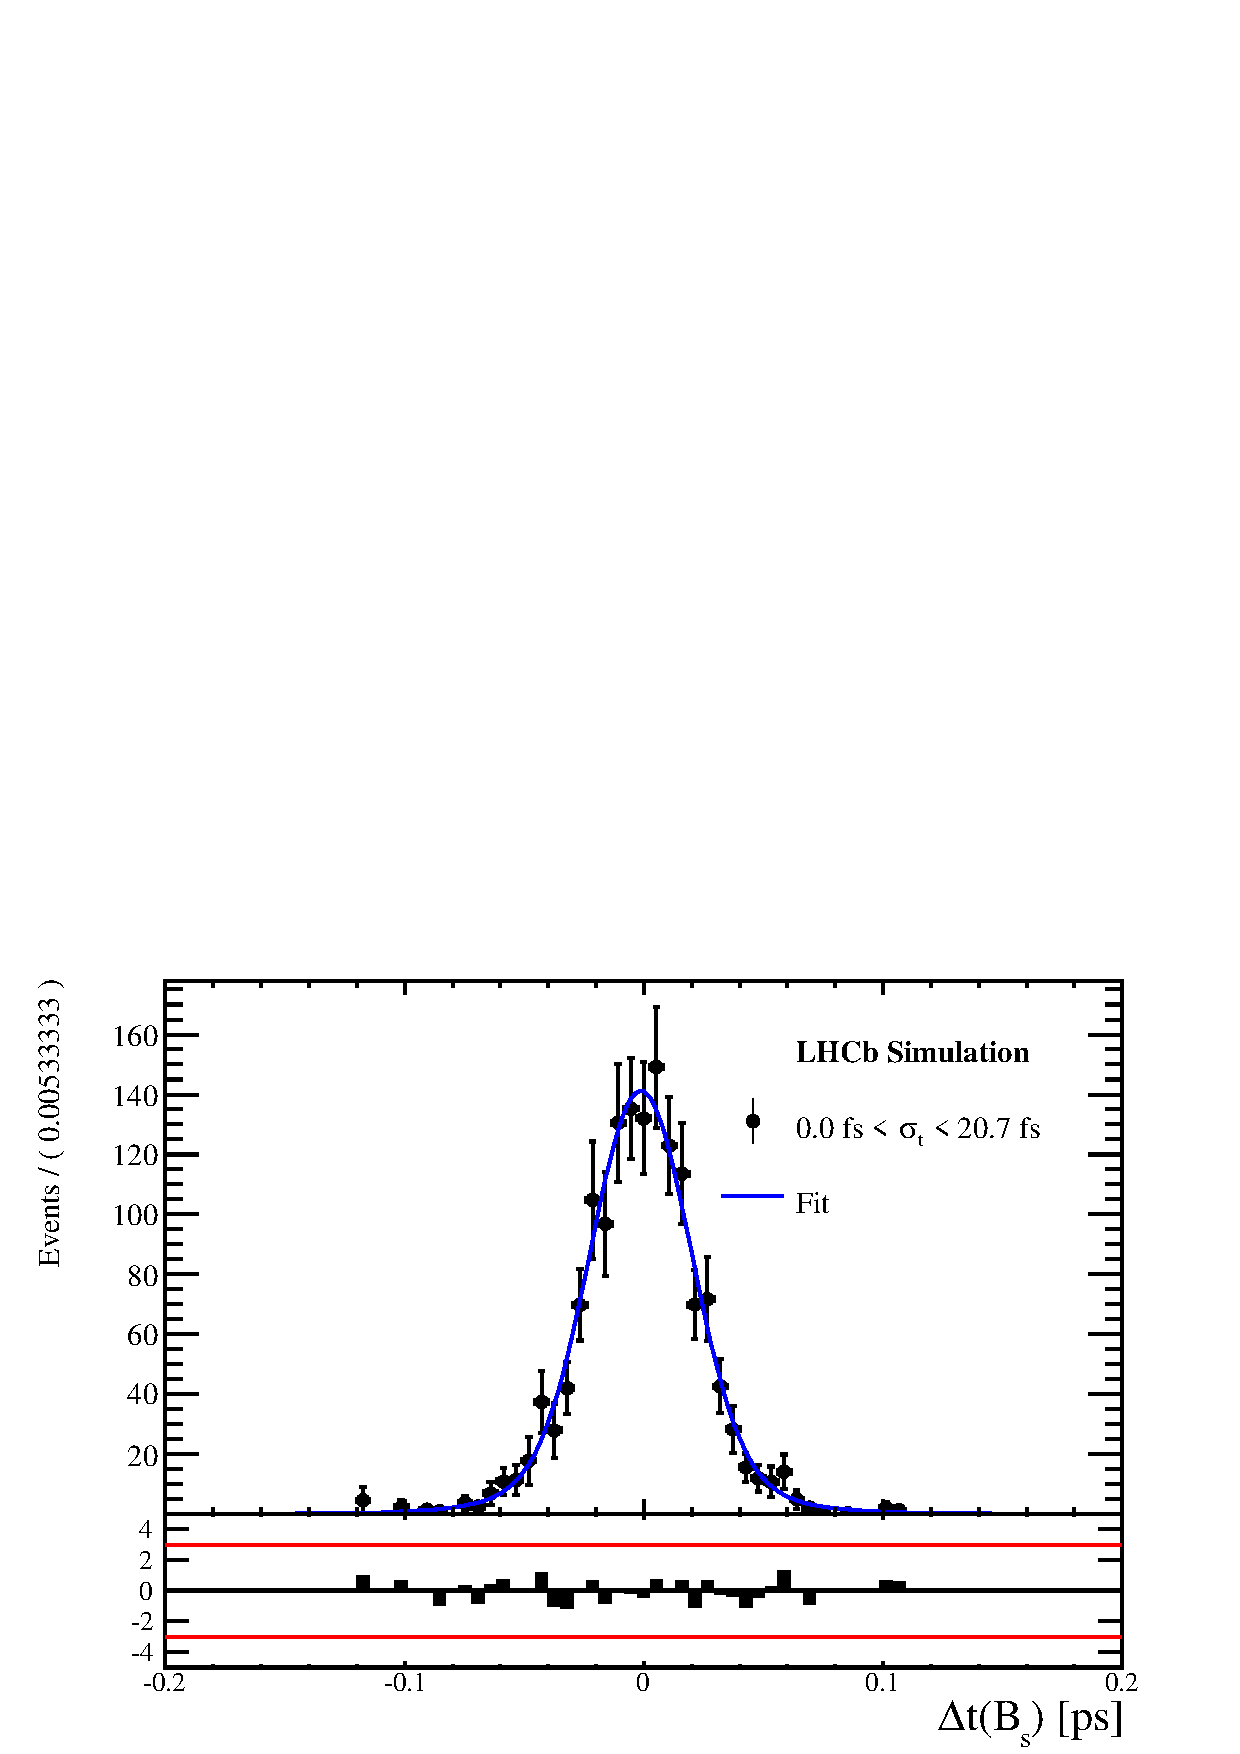
\includegraphics[height=!,width=0.4\textwidth]{figs/Resolution/SignalMC_bin_1.pdf}
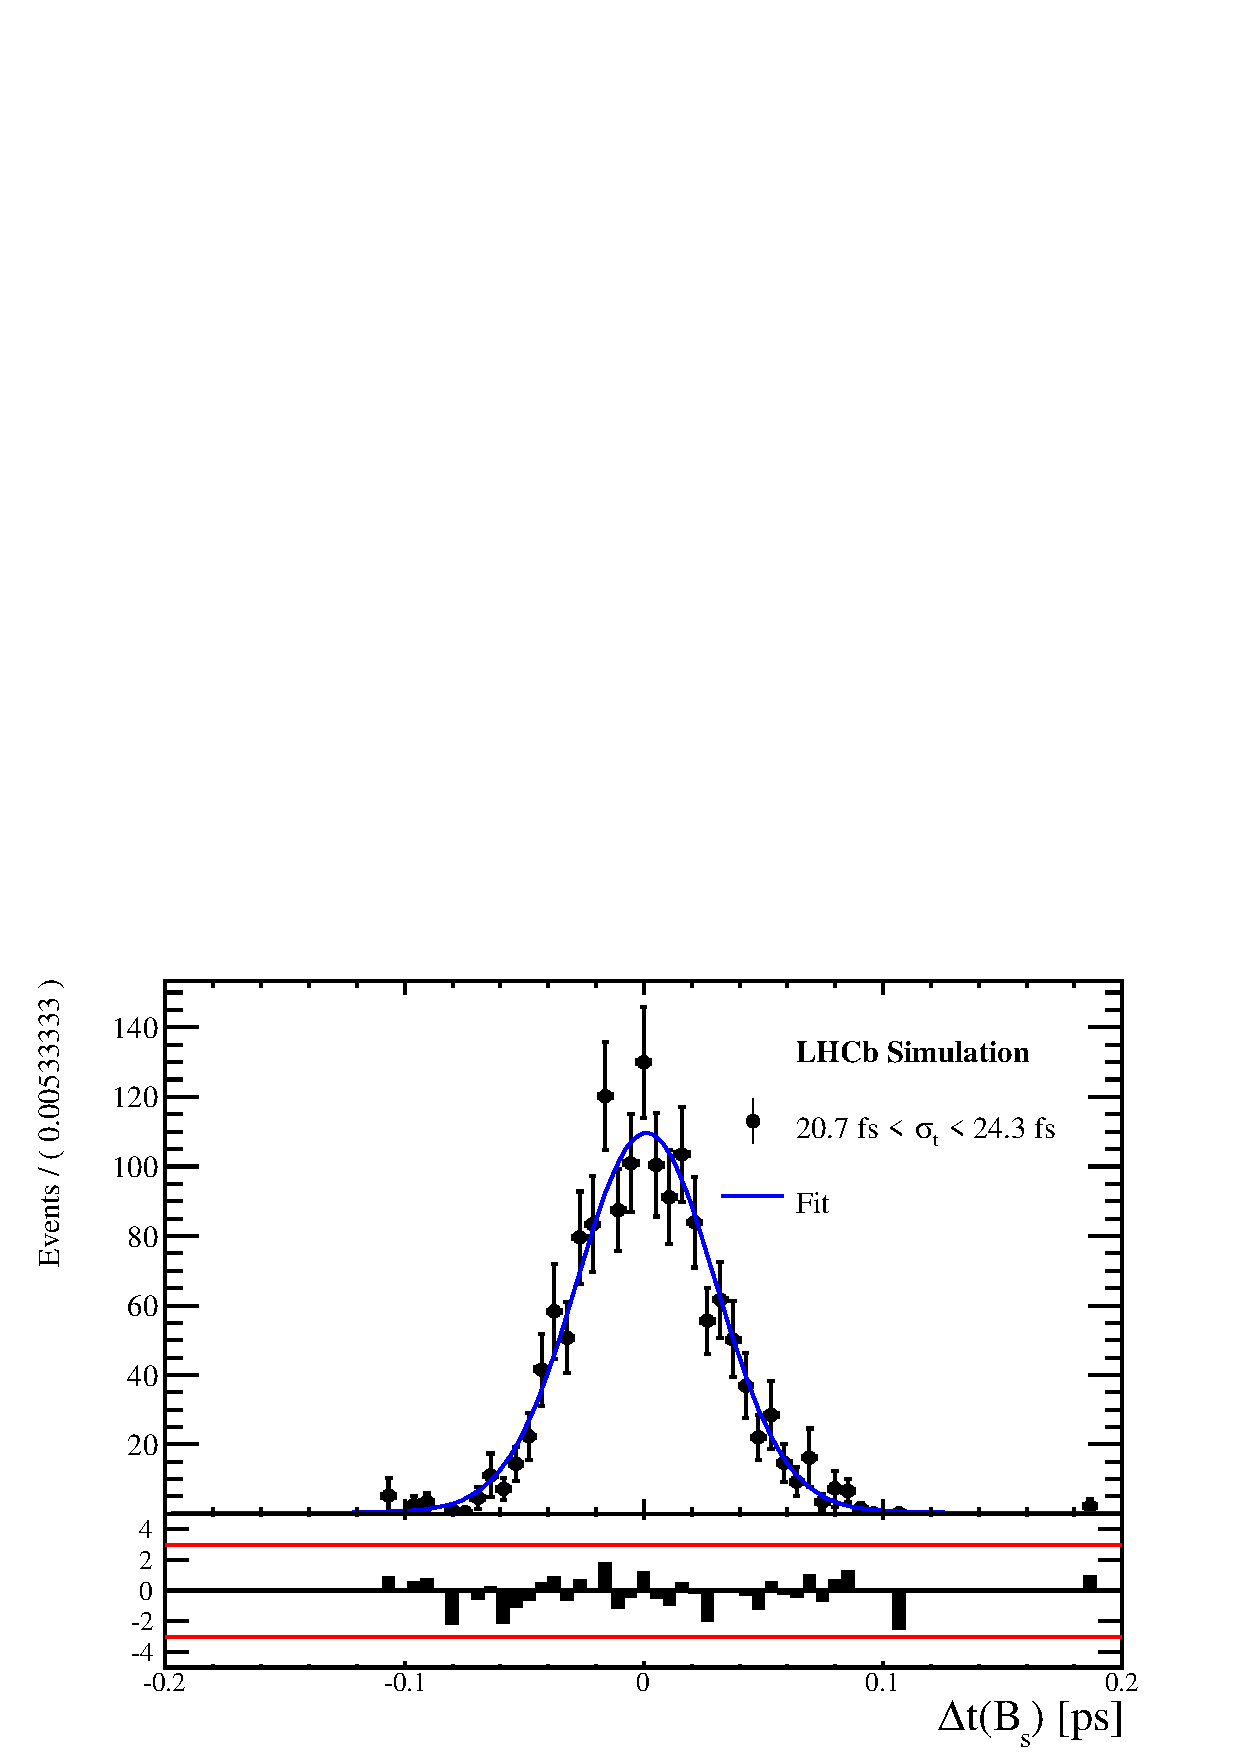
\includegraphics[height=!,width=0.4\textwidth]{figs/Resolution/SignalMC_bin_2.pdf}

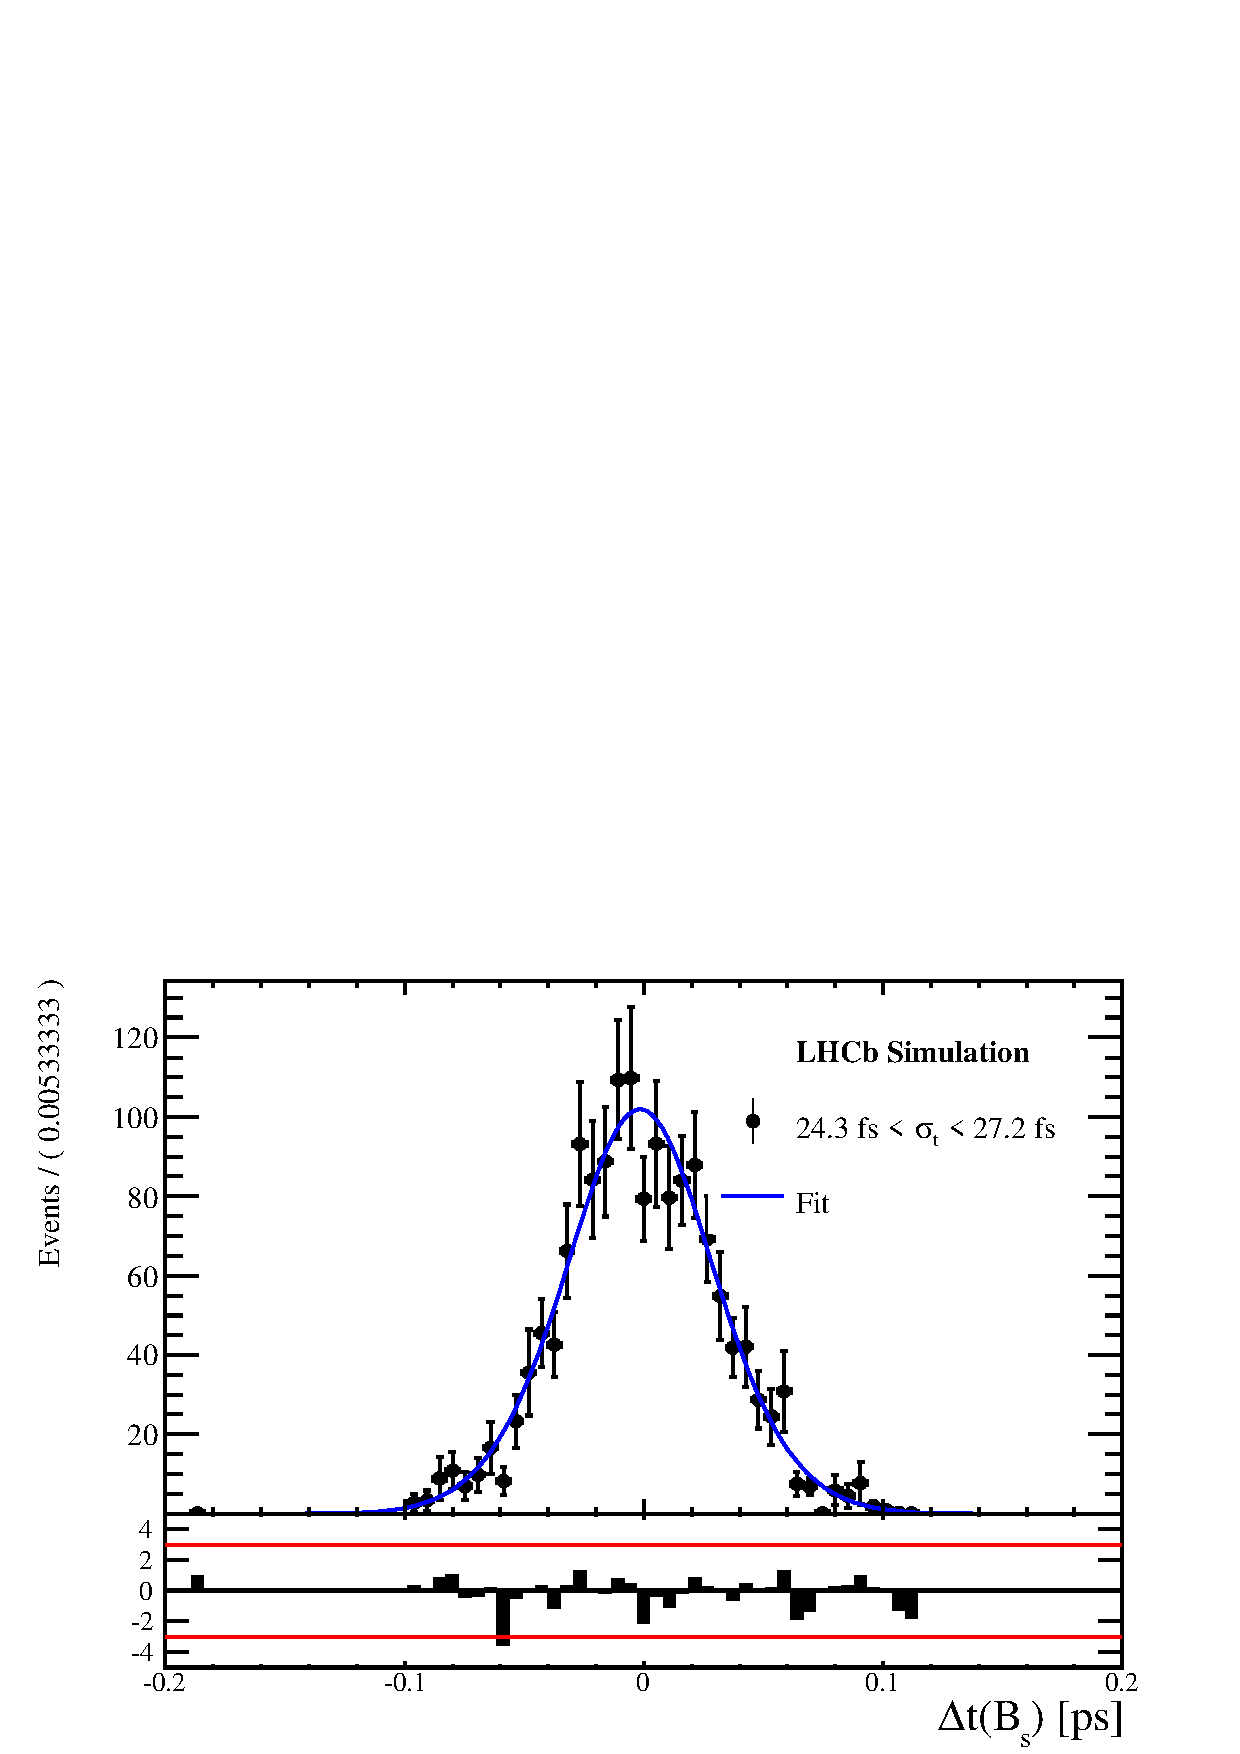
\includegraphics[height=!,width=0.4\textwidth]{figs/Resolution/SignalMC_bin_3.pdf}
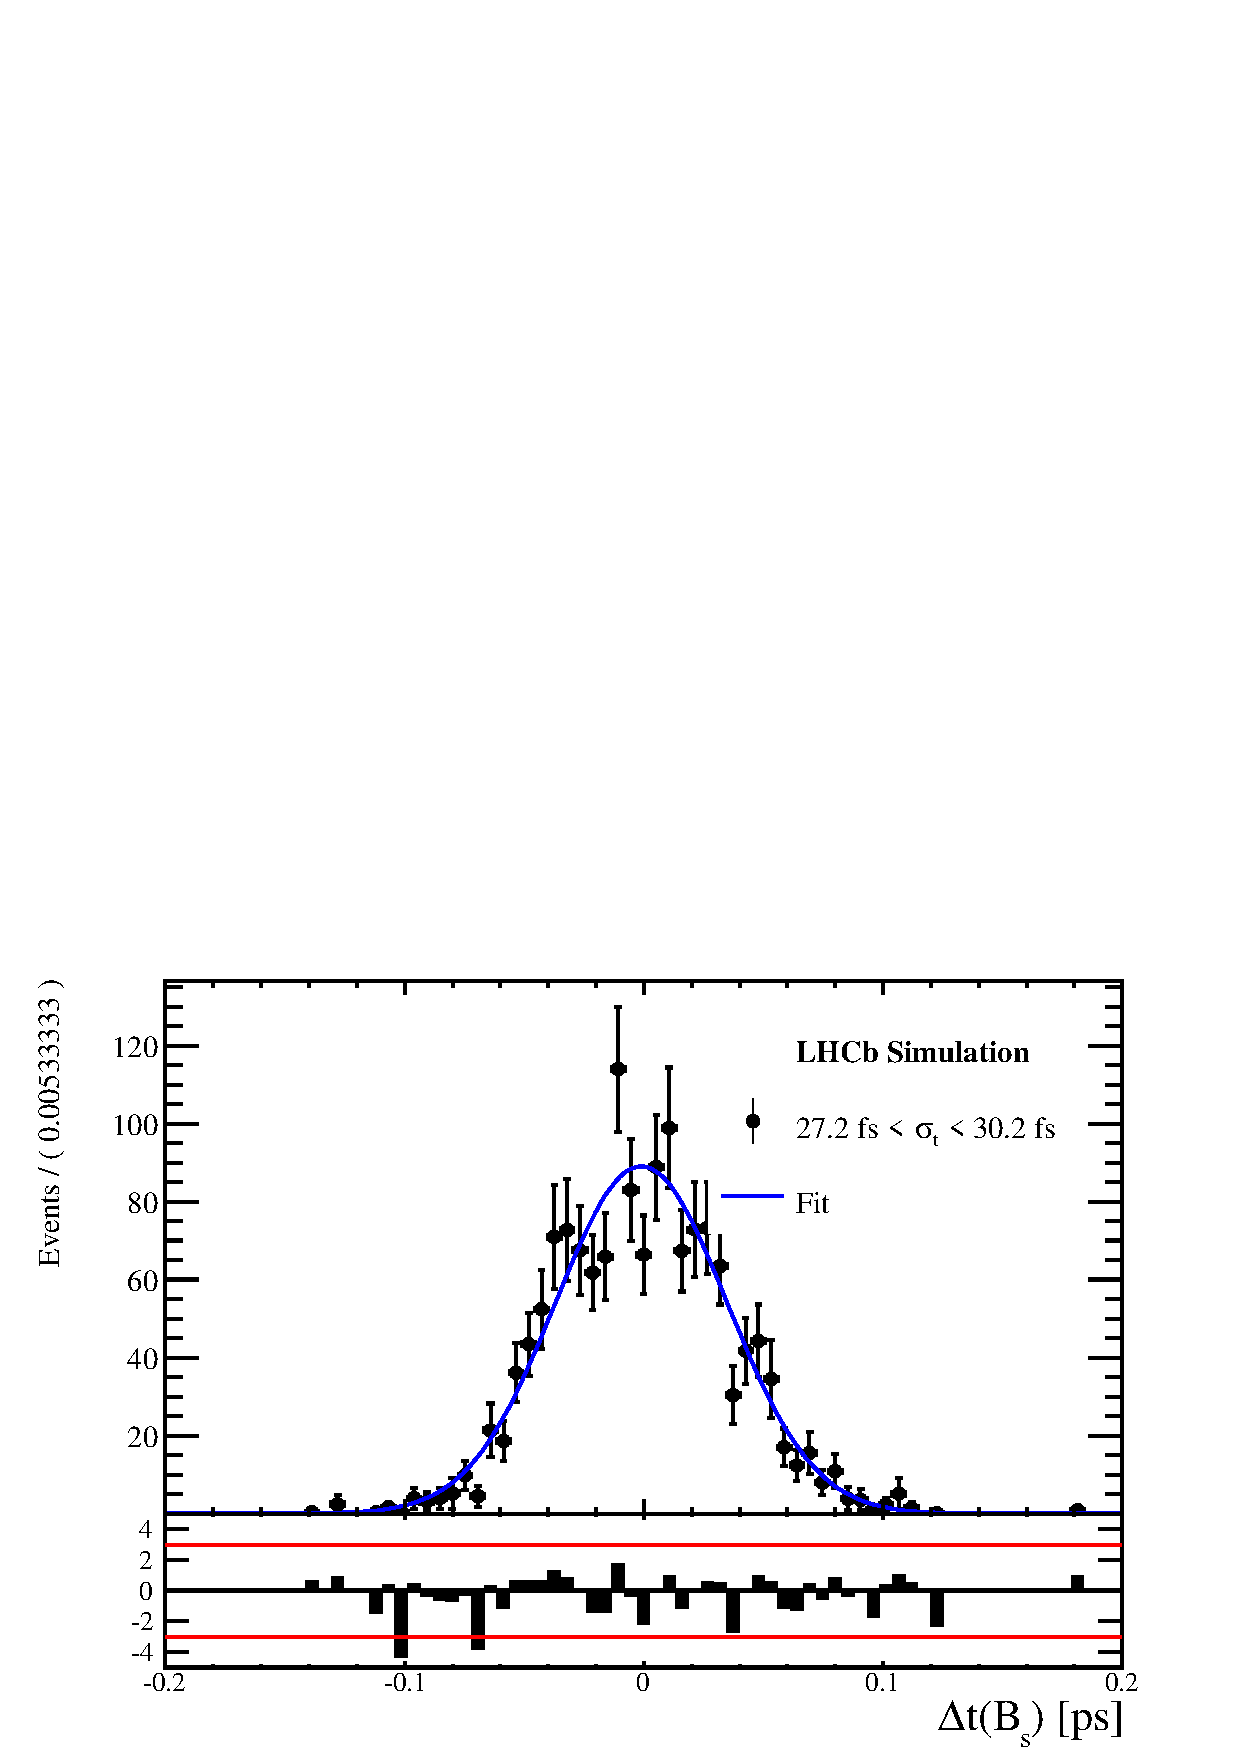
\includegraphics[height=!,width=0.4\textwidth]{figs/Resolution/SignalMC_bin_4.pdf}

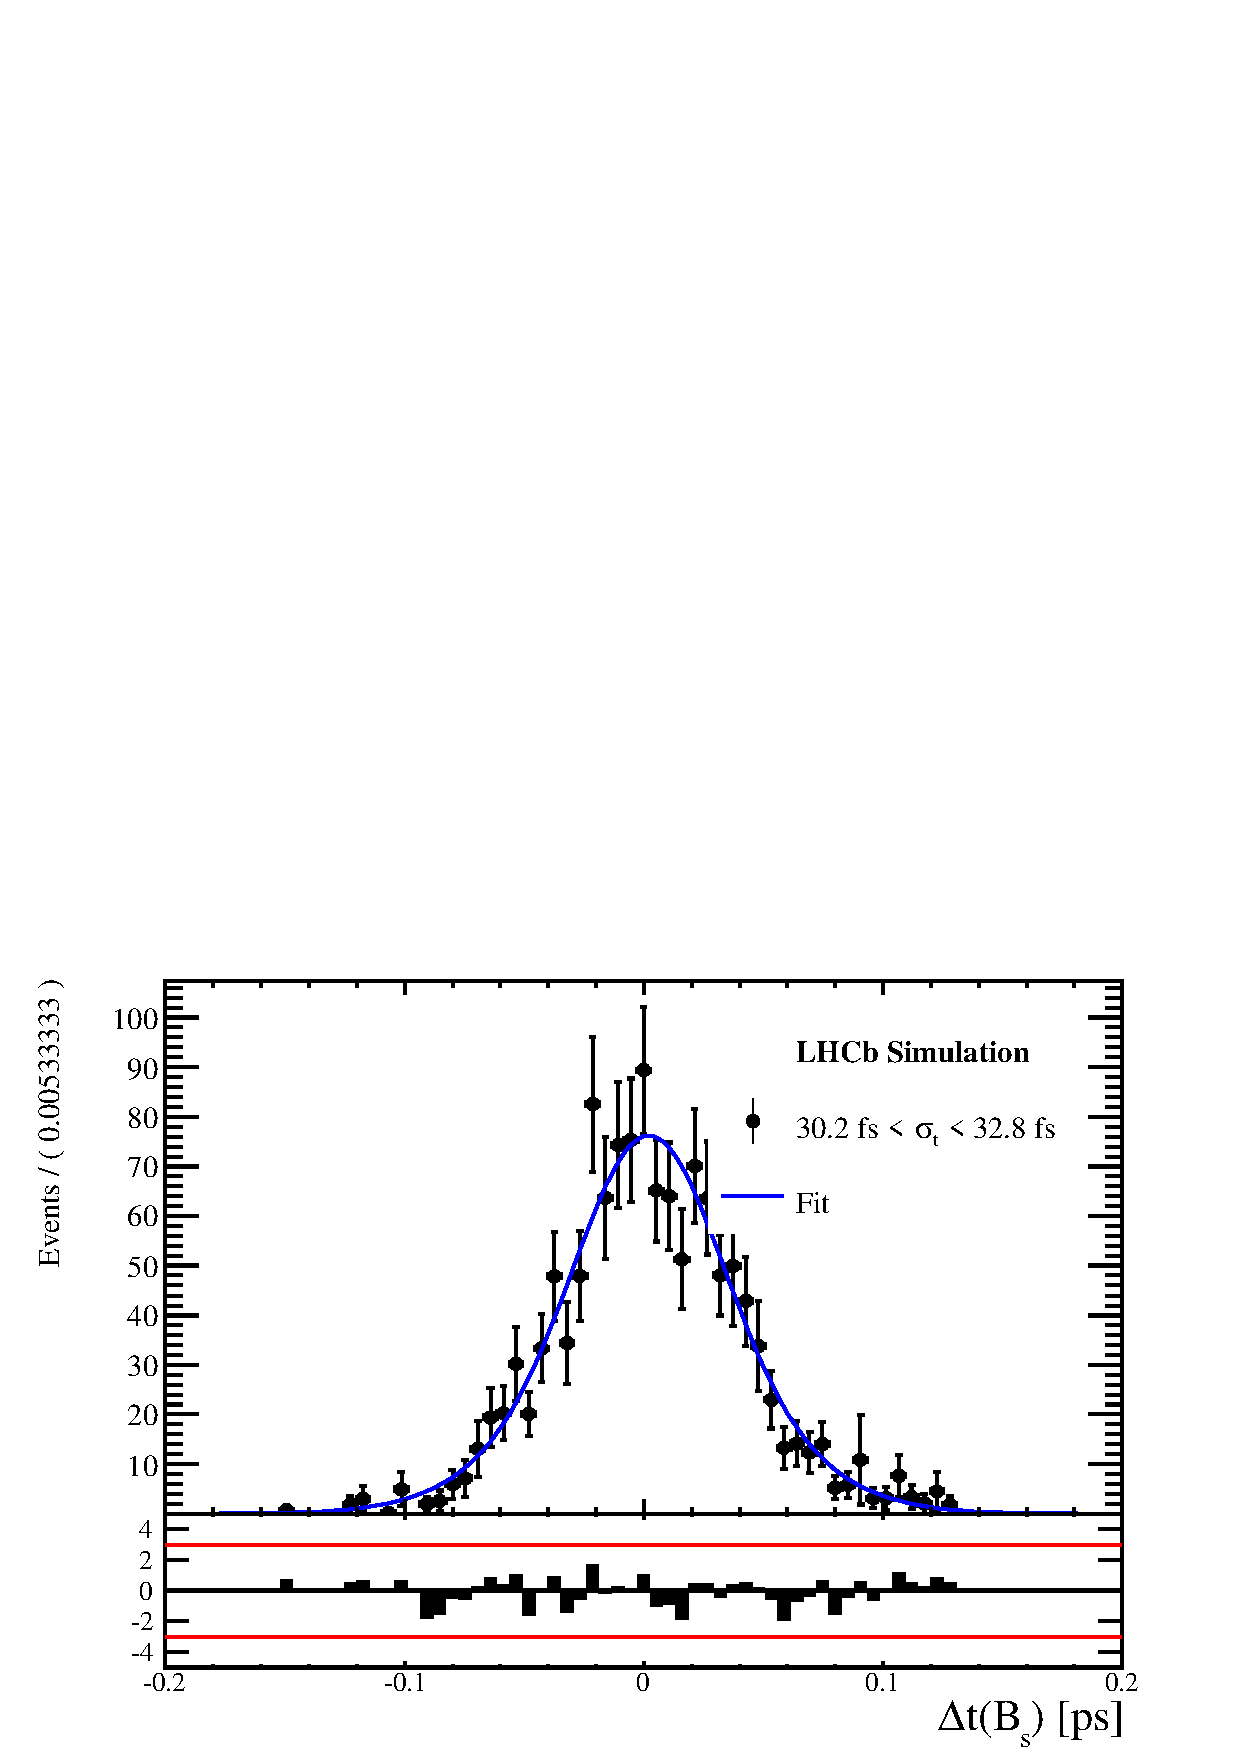
\includegraphics[height=!,width=0.4\textwidth]{figs/Resolution/SignalMC_bin_5.pdf}
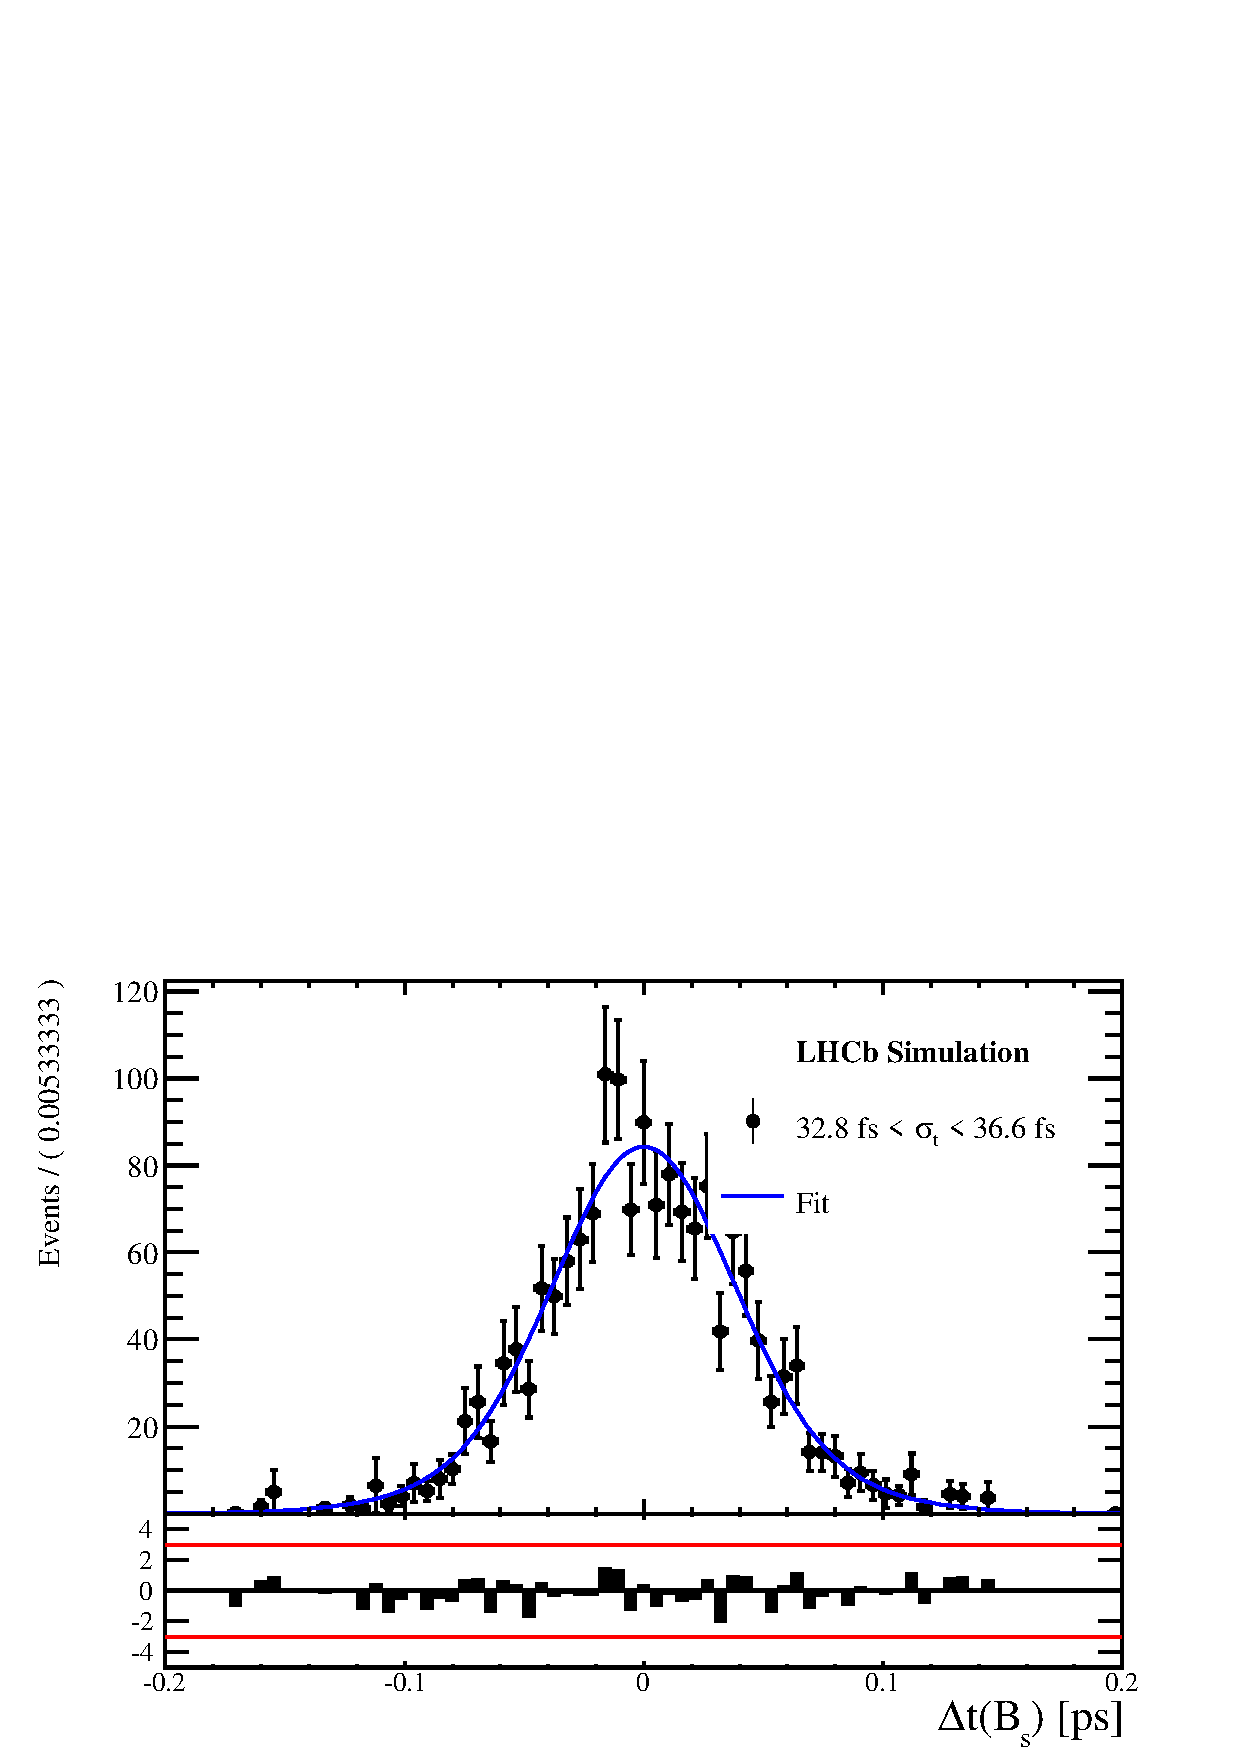
\includegraphics[height=!,width=0.4\textwidth]{figs/Resolution/SignalMC_bin_6.pdf}

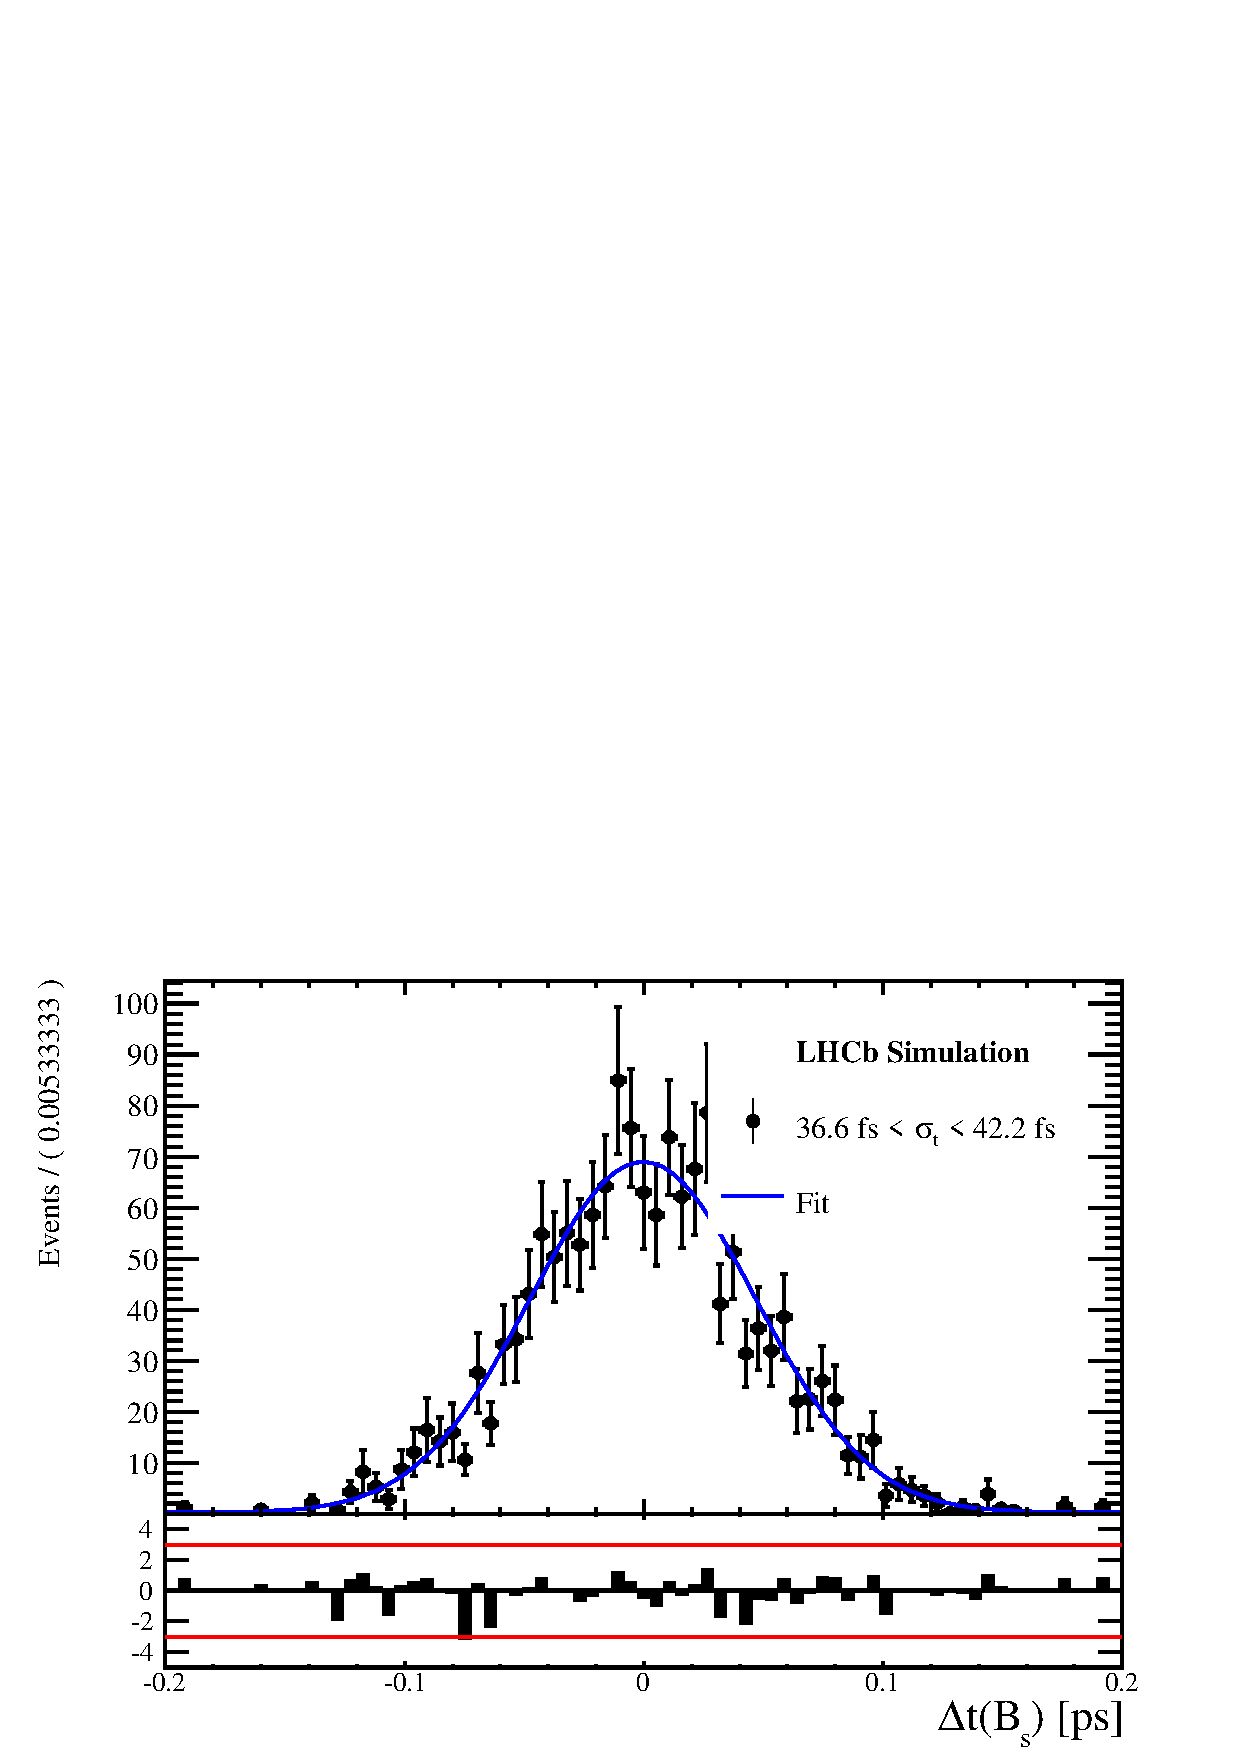
\includegraphics[height=!,width=0.4\textwidth]{figs/Resolution/SignalMC_bin_7.pdf}
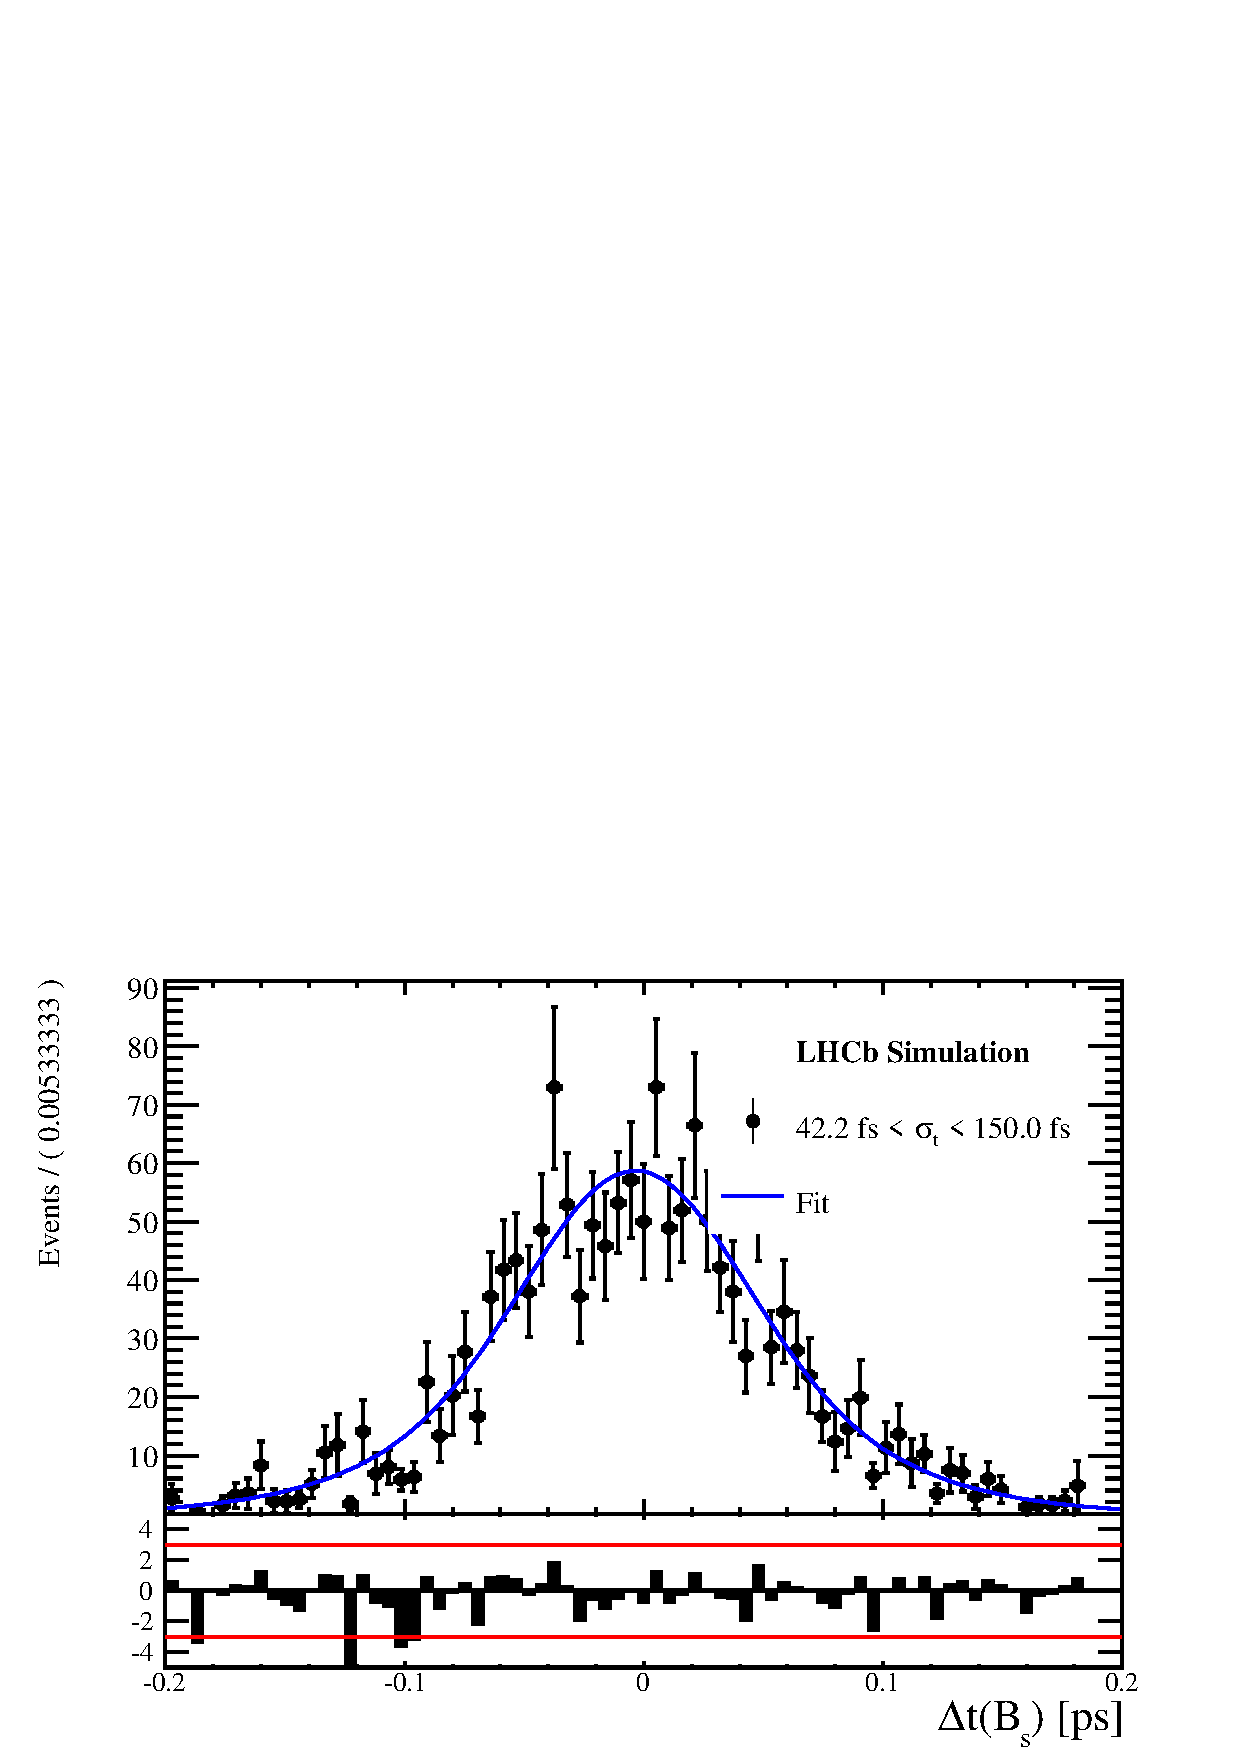
\includegraphics[height=!,width=0.4\textwidth]{figs/Resolution/SignalMC_bin_8.pdf}
\caption{Difference of the true and measured decay time of $\Bs\to\Ds\kaon\pion\pion$ MC candidates in bins of the per-event decay time error estimate..}
\label{fig:}
\end{figure}

\input{tables/Resolution/ResoTable_MC.txt}

\clearpage

\begin{figure}[h]
\centering
\includegraphics[height=!,width=0.4\textwidth]{figs/Resolution/SignalData_bin_1.pdf}
\includegraphics[height=!,width=0.4\textwidth]{figs/Resolution/SignalData_bin_2.pdf}

\includegraphics[height=!,width=0.4\textwidth]{figs/Resolution/SignalData_bin_3.pdf}
\includegraphics[height=!,width=0.4\textwidth]{figs/Resolution/SignalData_bin_4.pdf}

\includegraphics[height=!,width=0.4\textwidth]{figs/Resolution/SignalData_bin_5.pdf}
\includegraphics[height=!,width=0.4\textwidth]{figs/Resolution/SignalData_bin_6.pdf}

\includegraphics[height=!,width=0.4\textwidth]{figs/Resolution/SignalData_bin_7.pdf}
\includegraphics[height=!,width=0.4\textwidth]{figs/Resolution/SignalData_bin_8.pdf}
\caption{Decay-time distribution for fake $B_s$ candidates from promptly produced $D_s$ candidates, combined with random prompt $K\pi\pi$ bachelor tracks, for bins in the per-event decay time error estimate.}
\label{fig:}
\end{figure}

\input{tables/Resolution/ResoTable_Data.txt}

